\section{EDID subsystem}
\label{sec:edid}

As large parts of the system are highly-dependent on the format of the incoming video data, sensor modules are required to implement an \gls{edid}-like structure which can be transferred over the \gls{ddc} channel to notify downstream components about the video format used by the image sensor so that the data can be capture correctly.

The proof-of-concept contains a subset of \gls{edid} fields specifically selected for use by image sensors to describe their capabilities. Unlike regular \gls{edid}, where the video source probes the video sink for its capabilities, the data is stored on the video source (the image sensor) and is retrieved by the video sink (the main camera body). In addition to ensuring the camera hardware is configured correctly for image capture, the \gls{edid} data can also be appended to the captured image files as metadata to aid in the storage and archival process. The following sections detail the separate blocks which make up a full example \gls{edid} for the OV7670.

\subsection{Manufacturer and product ID}
The manufacturer and product ID block contains purely informational metadata required for keeping track of which sensor module is installed. This data is particularly useful in the archival process where a user might want to filter images which were taken with a specific camera or image sensor. Through a combination of the manufacturer ID, product ID and serial number, each image sensor is uniquely identifiable.  

\begin{table}[h]
    \begin{tabular}{lll}
        Field               & Block address             & Value             \\
        \hline
        Manufacturer ID     & \multirow{5}{*}{0x08}     & OVT               \\
        Product ID          &                           & 7670              \\
        Serial number       &                           & 12345             \\
        Week / year         &                           & Week 9, Year 2016 \\
    \end{tabular}
\end{table}

\subsection{Header information}
The header information block is used only to check that the sensor module implements a compatible \gls{edid} version supported by the camera body. \gls{edid} version 1.4 is currently the most widely supported version at the time of writing.

\begin{table}[h]
    \begin{tabular}{lll}
        Field               & Block address             & Value             \\
        \hline
        EDID version        & 0x12                      & Version 1.4       \\
    \end{tabular}
\end{table}

\subsection{Sensor parameters}
The sensor parameters block contains details on the physical dimensions and interface of the image sensor. For a proof-of-concept system the sensor parameters block is not terribly important, however in a real system the sensor dimensions (referred to here as the \textit{Screen size} to comply with the \gls{edid} specification) could be used to calculate whether the image circle produced by a lens will cover the sensor plane, or will only partially expose the sensor, resulting in vignetting around the corners. As \gls{edid} is really intended for use with displays there are some clear discrepancies when used to describe an image sensor. \textit{Signal type} is guaranteed to be digital --- this field is a relic from when \gls{edid} was used with \gls{crt} displays. Apart from being used here to refer to the active area of the sensor, \textit{Screen size} measured centimetres and only allows for integers. The pixels on image sensors are far smaller, and thus millimetres would be a more suitable unit of measurement. \textit{Colour bit depth} is a very important field as higher-end image sensors tend to have higher-resolution \glspl{adc}.

\begin{table}[h]
    \begin{tabular}{lll}
        Field               & Block address             & Value                                         \\
        \hline
        Signal type         & \multirow{4}{*}{0x14}     & Digital                                       \\
        Colour bit depth    &                           & \SI{8}{\bit}                                 \\
        Interface           &                           & DVI                                           \\
        Screen size         &                           & \SI{2}{\centi\metre} x  \SI{1}{\centi\metre}  \\ 
    \end{tabular}
\end{table}

\subsection{Established timings}
The established timings block is used to mark which common VESA output resolutions are supported. The information here is misleading as the OV7670 actually only outputs at \SI{30}{\hertz}, however only the resolutions detailed in the VESA Display Monitor Timings specification can be used here \cite{video_timing}. As Image sensors vary wildly from regular displays in terms of resolution and framerate, it is unlikely that the established timings block is of any use.

\begin{table}[h]
    \begin{tabular}{lll}
        Field               & Block address             & Value                         \\
        \hline
        Established timings & 0x23                      & 640 x 480 @ \SI{60}{\hertz}   \\
    \end{tabular}
\end{table}

\subsection{Detailed timings}
\Gls{edid} also includes a detailed timings block where manufacturers can specify custom timings which are not part of the VESA Display Monitor Timings standard. This block is absolutely critical for image sensors with non-standard timings. As the video data is not being used to drive a monitor directly, there are no constraints on video timings other than ensuring that the blanking period is sufficiently long for transferring each line into the framebuffer.

\begin{table}[h]
    \begin{tabular}{lll}
        Field               & Block address             & Value                 \\
        \hline
        Pixel clock         & \multirow{9}{*}{0x36}     & \SI{12}{\mega\hertz}  \\
        H. active pixels    &                           & 640                   \\
        H. blanking pixels  &                           & 160                   \\
        V. active pixels    &                           & 480                   \\ 
        V. blanking pixels  &                           & 45                    \\
        H. sync width       &                           & 96                    \\
        H. front porch      &                           & 16                    \\
        V. sync width       &                           & 2                     \\
        V. front porch      &                           & 10                    \\
    \end{tabular}
\end{table}

\subsection{Monitor description}
To supplement the manufacturer and product ID block, the monitor description block can be used to specify various human-readable tags such as the product or manufacturer name. Single-lens reflex cameras typically feature a `through-the-lens' viewfinder, whereby a mirror is used to direct light away from the sensor and into the viewfinder for composition, only lifting up to allow the sensor to be exposed when the shutter release is pressed. As it is only possible to tell which sensor was installed after capturing an image, the sensor name can be projected on the viewfinder for at-a-glance information. A mockup of the viewfinder is illustrated in Figure \ref{fig:viewfinder}. Like the manufacturer and product ID block, this data can be embedded into the final image as metadata which is very useful in the storage and archival process.

\begin{table}[h]
    \begin{tabular}{lll}
        Field               & Block address             & Value             \\
        \hline
        Data type tag       & \multirow{2}{*}{0x48}     & Product name      \\
        Product name        &                           & OV7670            \\
    \end{tabular}
\end{table}

\begin{figure}
  \centering
  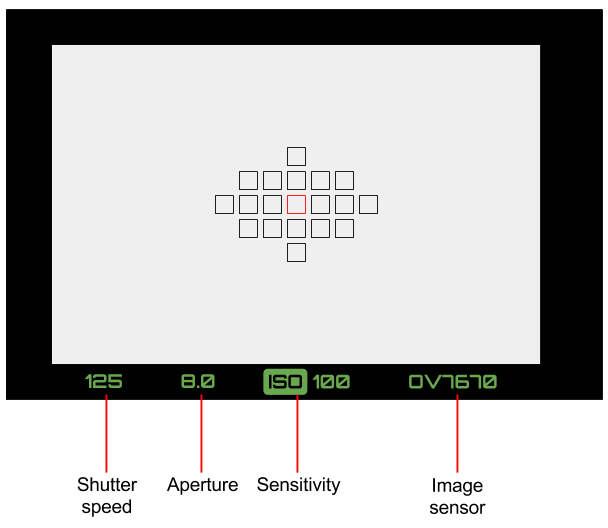
\includegraphics[width=0.7\textwidth]{./img/viewfinder.png}
  \caption{Mockup showing how the currently-installed sensor can be projected onto the viewfinder.}
  \label{fig:viewfinder}
\end{figure}

\subsection{Vendor extensions}
\gls{edid} also allows for vendor-specific extension blocks to be used which can be utilised here to add additional sensor-specific functionality. In order to add colour back to the RAW image the \gls{cfa} pattern must be known ahead of time in order to de-mosaic the image. While most image sensors implement the standard Bayer pattern, some image sensors, such as the Fuji X-Trans line, opt for exotic patterns which supposedly boast higher image quality. De-mosaicing an image with an incorrect \gls{cfa} pattern will result in unrealistic colour rendering, so it is essential that any part of the system which needs to perform de-mosaicing has an understanding of the \gls{cfa} pattern used on the image sensor. The most basic \gls{cfa} pattern is actually a 2 x 2 tiled array, so rather than storing the entire \gls{cfa} in the \gls{edid}, only the repeated tile needs to be stored.